% Official Frontiers supplementary material template version.
        \documentclass[utf8]{frontiers_suppmat}
        \usepackage{url,hyperref,lineno,microtype}
        \usepackage[onehalfspacing]{setspace}
        \usepackage{graphicx}

        \begin{document}
        \onecolumn
        \firstpage{1}

        \title[Supplementary Material]{{\helveticaitalic{Supplementary Material}}}

        \maketitle

        \section{Supplementary Tables}
        Supplementary tables are provided as \texttt{Supplementary\_Tables\_CTGFHT.xlsx} and as individual CSV files. Figure source-data tables are provided in the \texttt{source\_data} folder.

        \section{Supplementary Figures}
        \begin{figure}[h!]
              \begin{center}
              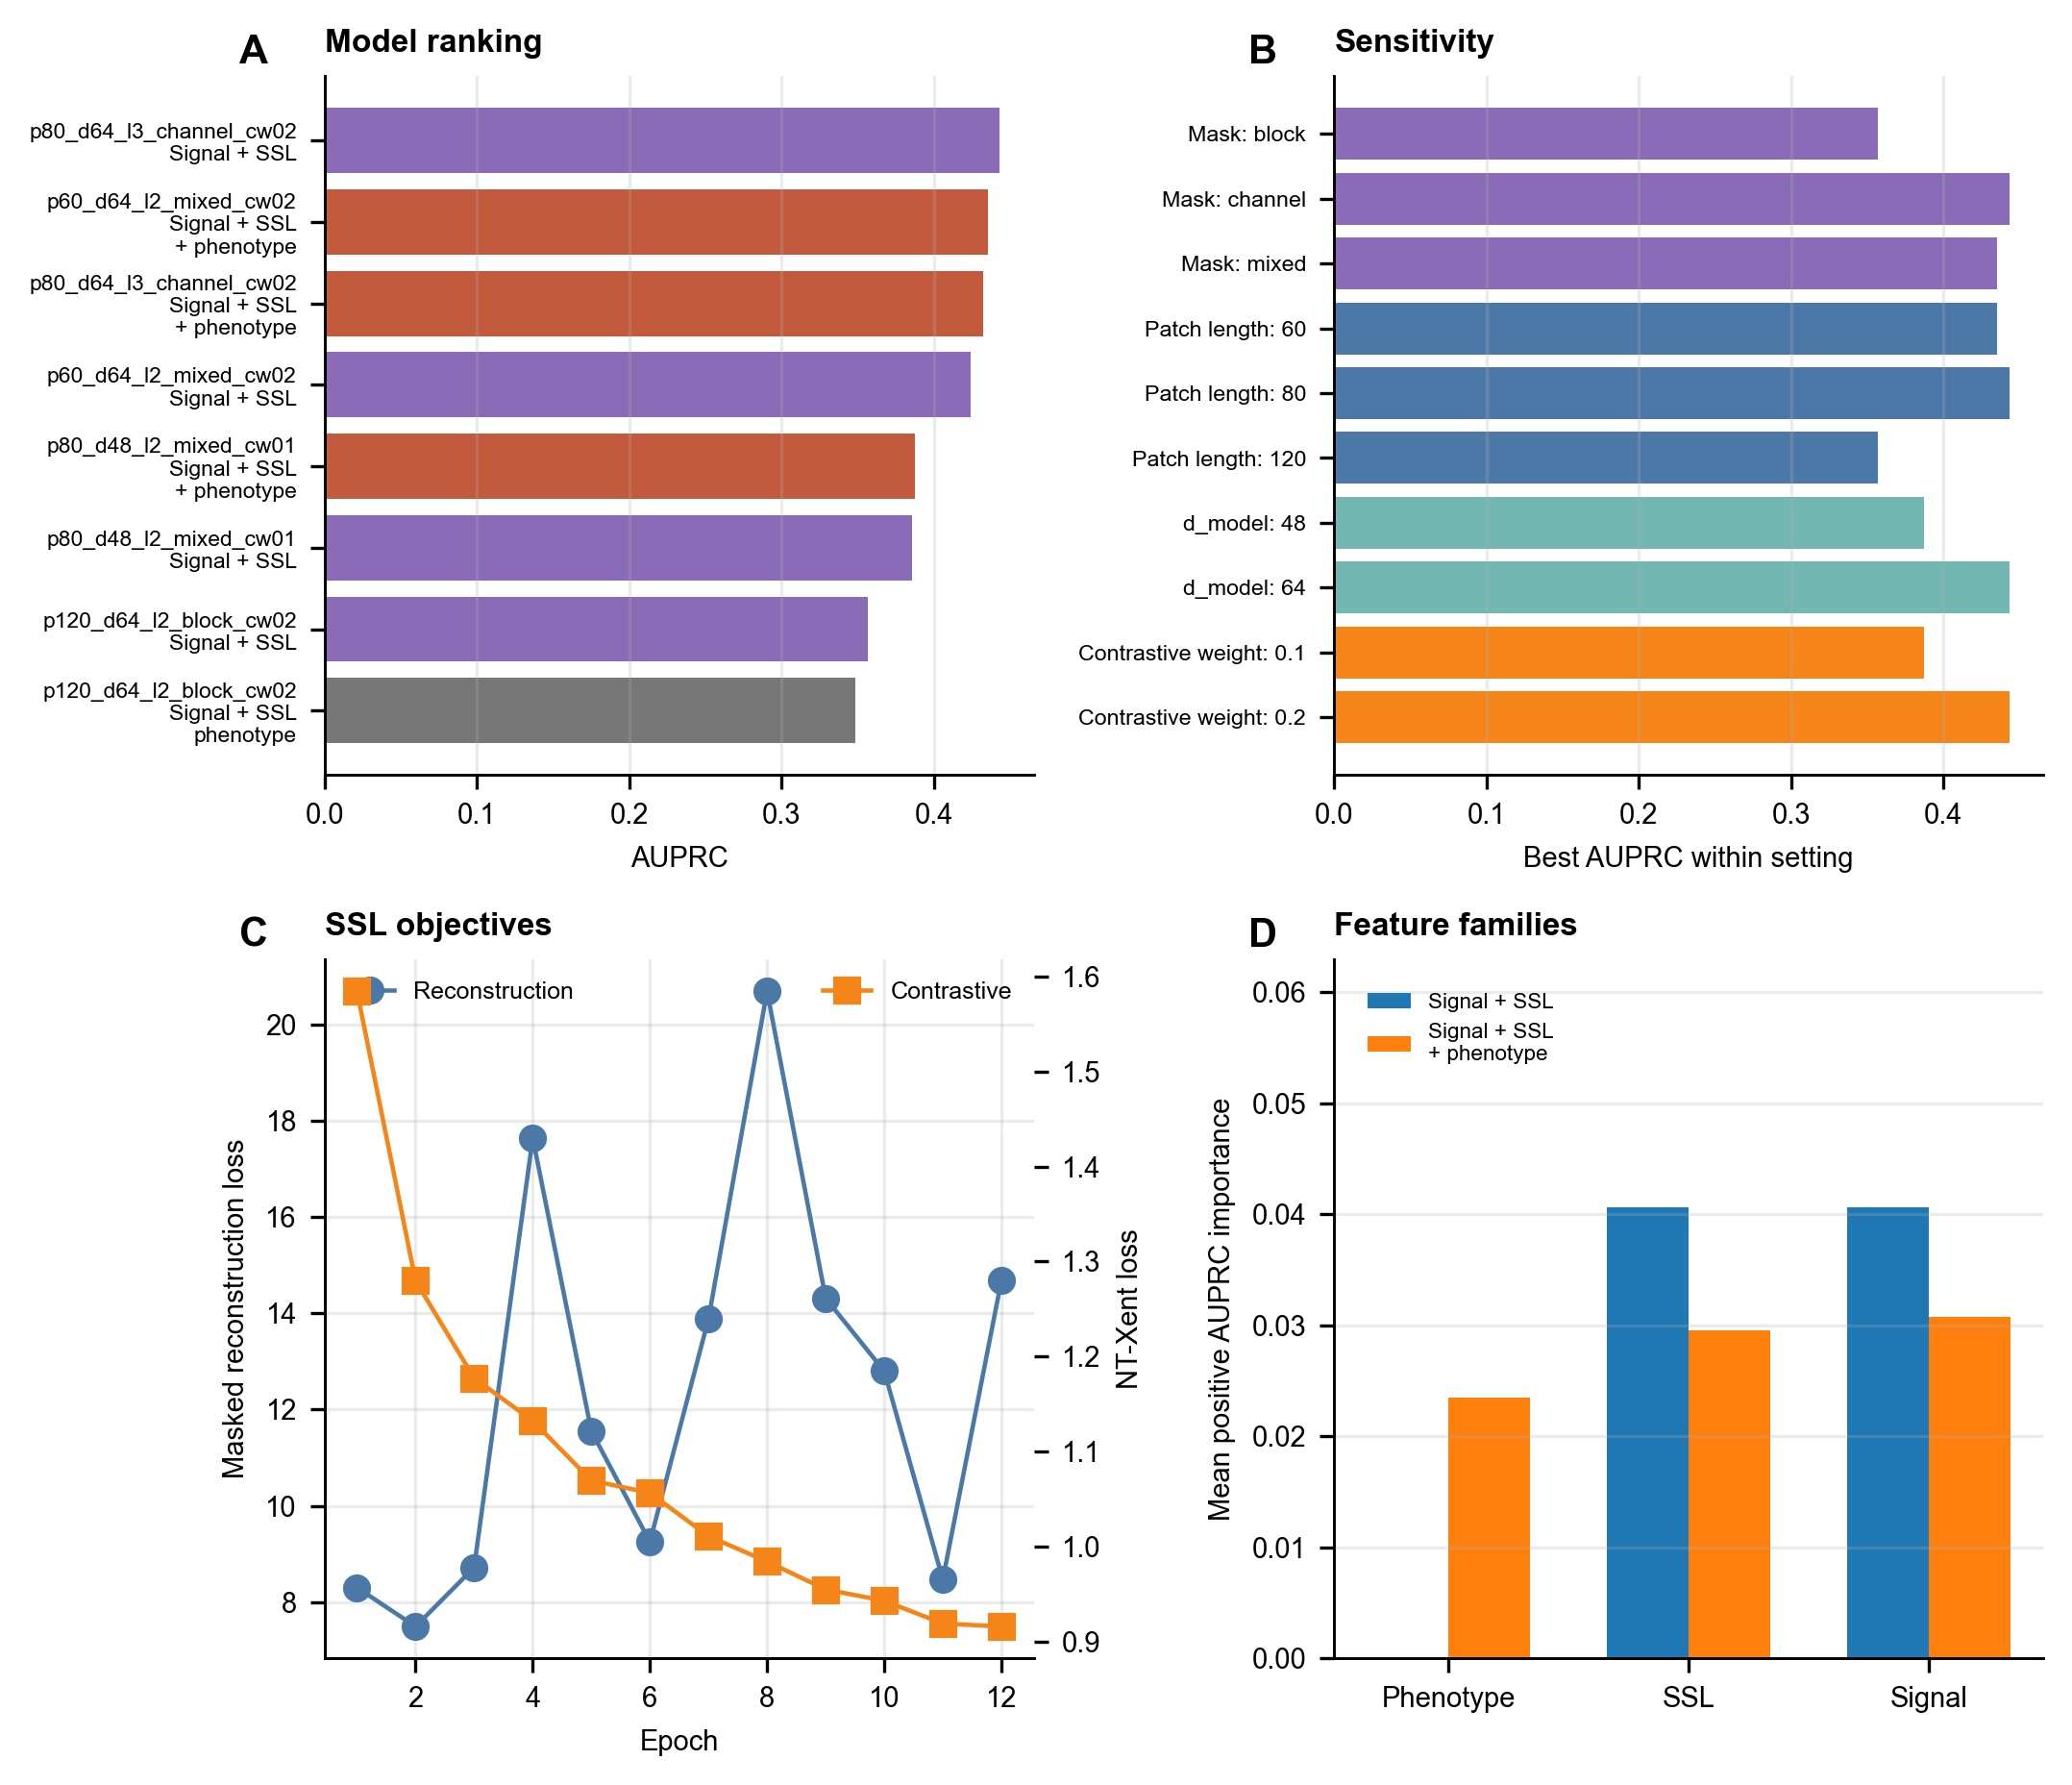
\includegraphics[width=\textwidth]{figures/Supplementary_Figure_S1_model_selection_and_sensitivity.jpg}
              \end{center}
              \caption{\textbf{AI model-selection and sensitivity panels for the transformer phenotyping workflow.}
Supplementary analyses of the self-supervised AI method layer. (A) Exploratory transformer configuration and feature-set combinations ranked by held-out AUPRC. (B) Sensitivity summary across masking strategy, patch length, model dimension and contrastive objective weight, using the best AUPRC observed within each setting. Because these panels use held-out performance for method exploration, they should not be interpreted as a locked independent model-selection experiment. (C) Training-objective trace for a selected-architecture refit, showing masked reconstruction loss and NT-Xent contrastive loss across epochs. (D) Feature-family contribution to AUPRC-based permutation importance for signal-plus-SSL and final phenotype-augmented models.}\label{fig:model_selection_sensitivity}
              \end{figure}

\begin{figure}[h!]
              \begin{center}
              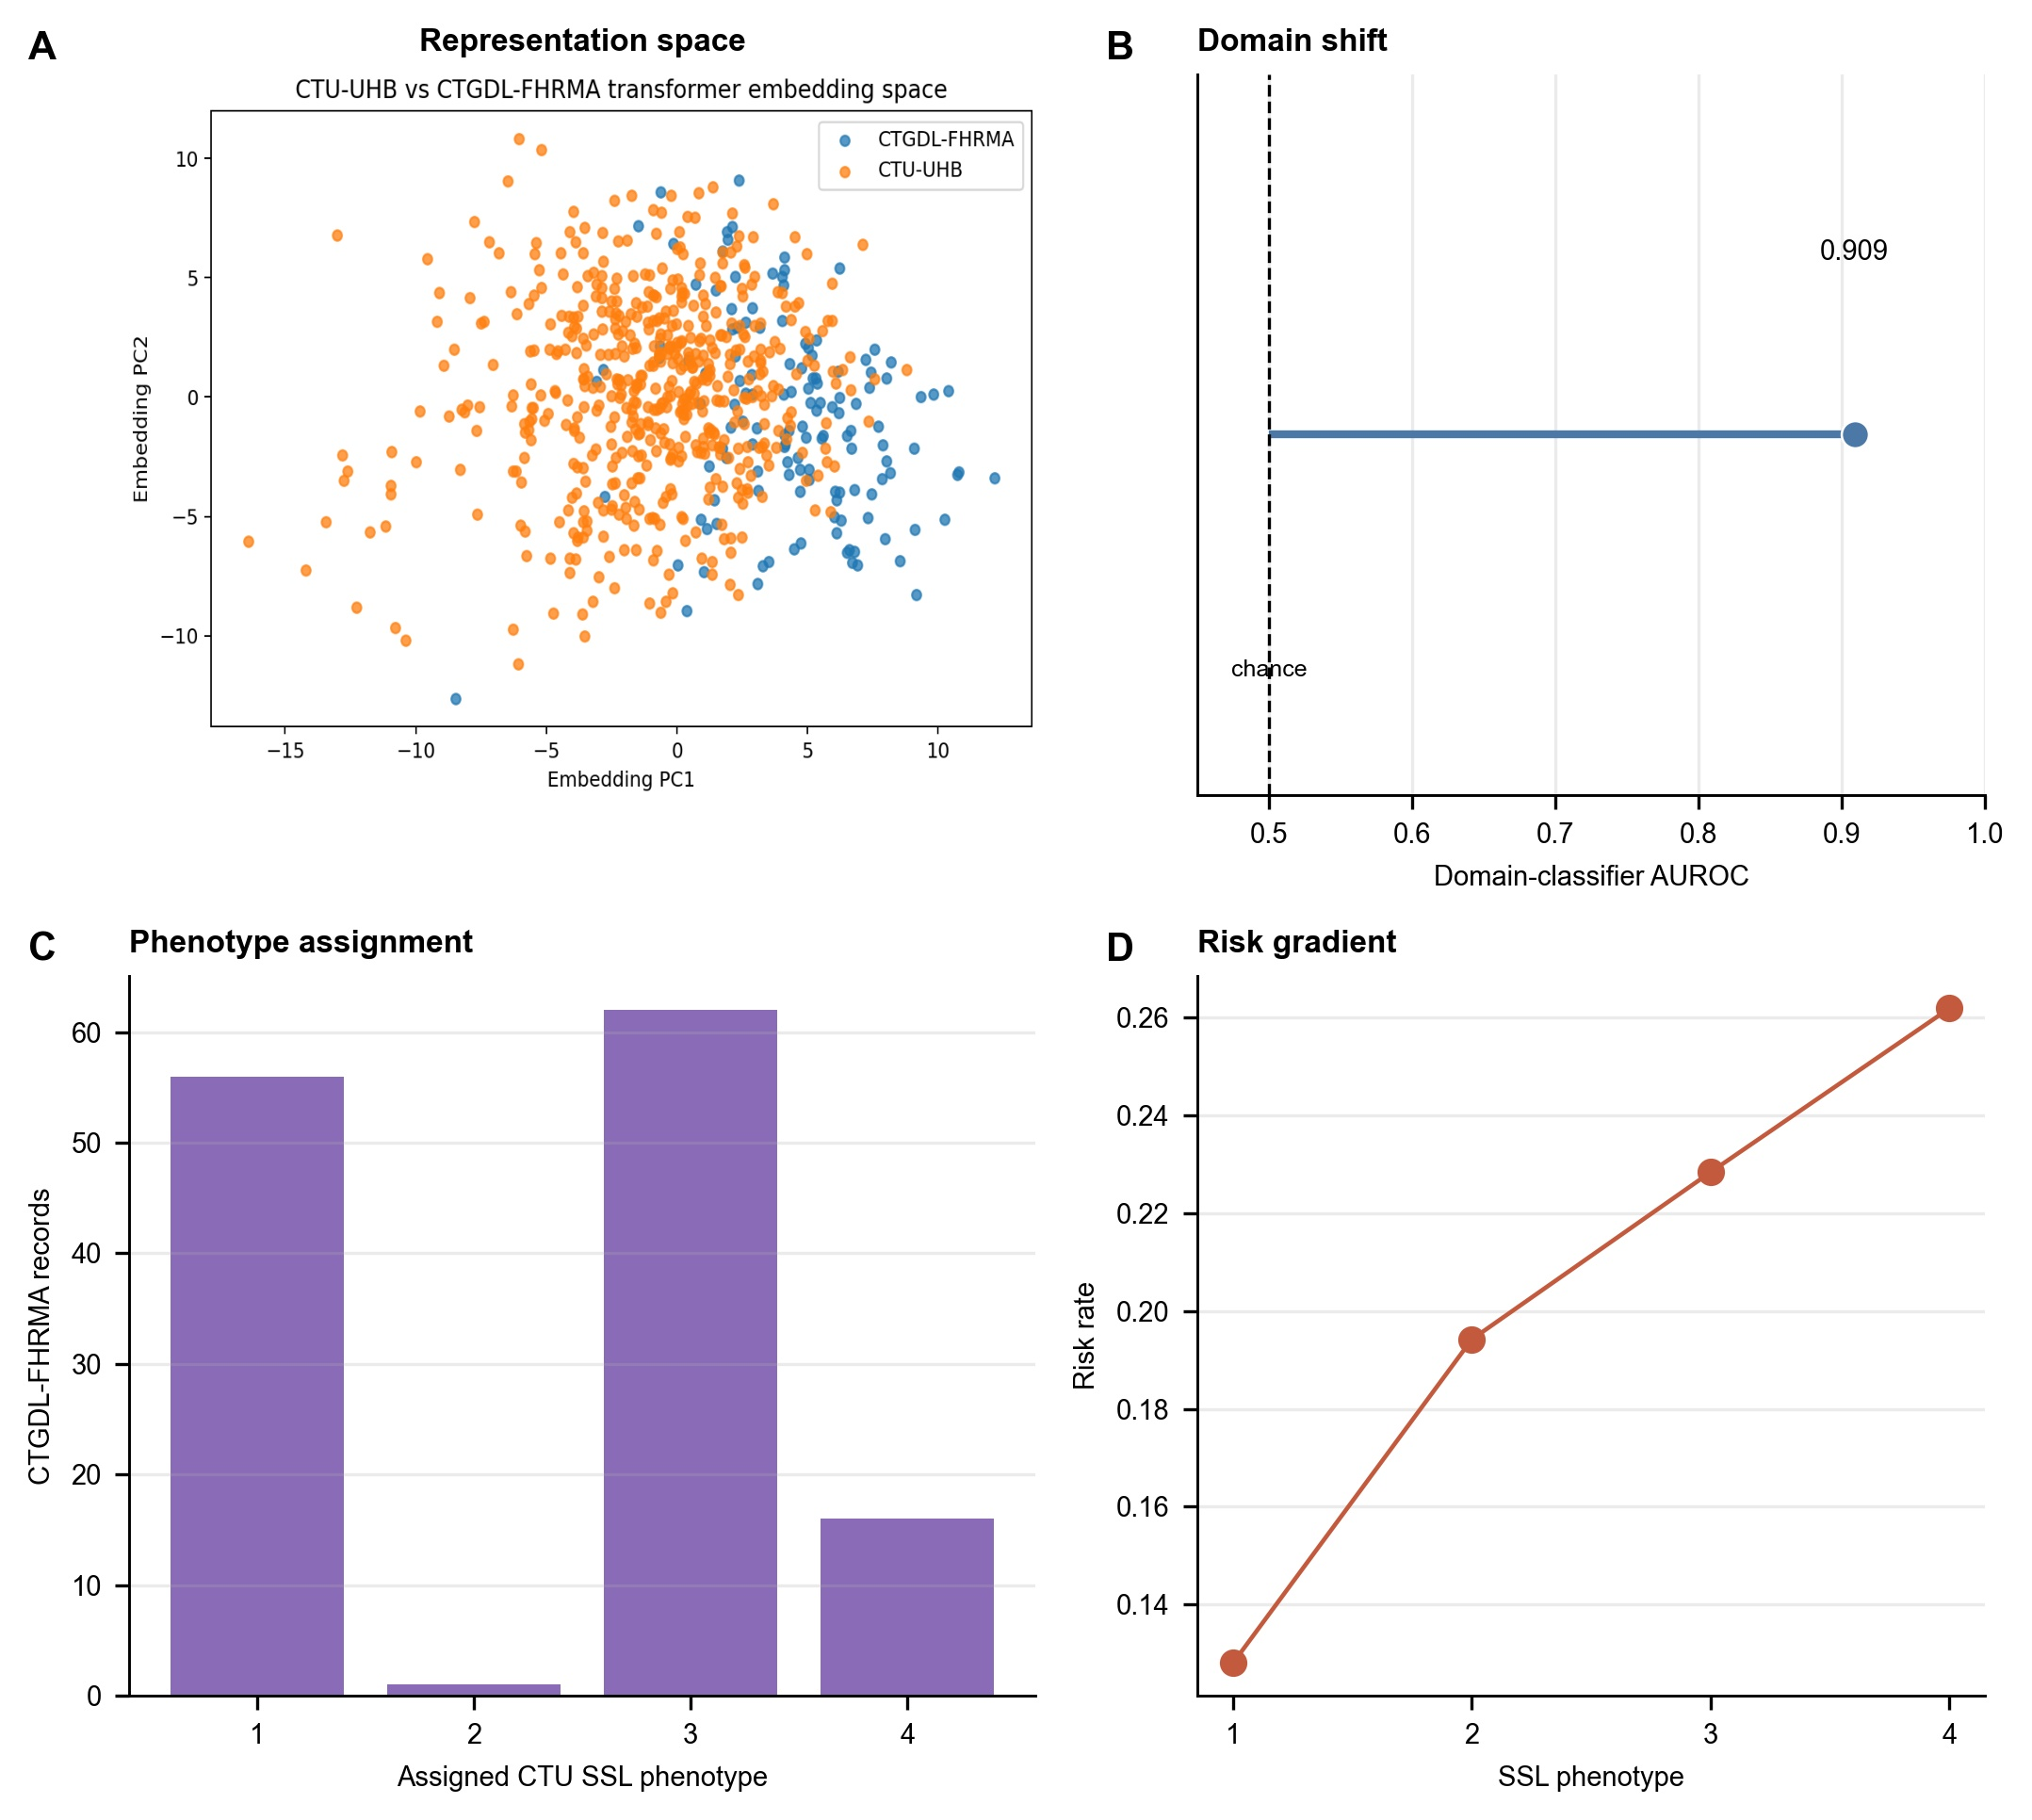
\includegraphics[width=\textwidth]{figures/Supplementary_Figure_S2_external_domain_shift.jpg}
              \end{center}
              \caption{\textbf{CTGDL-FHRMA supports external representation and domain-shift validation.}
External representation analysis using CTGDL-FHRMA records. Because external neonatal outcome labels were not used for CTGDL-FHRMA, this analysis is interpreted as external representation/domain-shift validation rather than external outcome validation. (A) Principal-component visualization of CTU-UHB and CTGDL-FHRMA transformer embeddings. (B) Domain separability quantified by a CTU-versus-CTGDL classifier. (C) CTGDL-FHRMA records assigned to CTU-derived SSL phenotypes. (D) CTU-UHB neonatal risk gradient across SSL phenotypes.}\label{fig:external}
              \end{figure}

        \end{document}
